\documentclass[12pt,reqno]{report}

\usepackage{amsmath, amssymb, amsfonts, amsbsy, amsthm, latexsym, graphicx, mathrsfs}
\usepackage{bbm}
\usepackage{bm}
\usepackage{forest}
\usepackage{caption}
% \usepackage{algorithm}
\usepackage{algorithm2e}
\usepackage{gensymb}
\usepackage{siunitx}
\usepackage{booktabs}
% \usepackage[table]{xcolor} % For coloring rows and columns
\usepackage{tikz}
\usepackage{hyperref}
\usepackage{listings}
\usepackage{xcolor}
\hypersetup{
    colorlinks=true,
    linkcolor=red,
    urlcolor=blue,
    citecolor=green,
}
\RestyleAlgo{ruled}

% \lstset{
%   basicstyle=\ttfamily,
%   keywordstyle=\color[rgb]{0.13, 0.13, 0.38}, % Keywords in navy blue
%   commentstyle=\color[rgb]{0.5, 0.5, 0.5}, % Comments in gray
%   stringstyle=\color[rgb]{0.63, 0.13, 0.13}, % Strings in dark red
%   backgroundcolor=\color[rgb]{0.95, 0.95, 0.95}, % Light gray background
%   frame=single,
%   breaklines=true,
%   showstringspaces=false,
% }

%New colors defined below
\definecolor{codegreen}{rgb}{0,0.6,0}
\definecolor{codegray}{rgb}{0.5,0.5,0.5}
\definecolor{codepurple}{rgb}{0.58,0,0.82}
\definecolor{backcolour}{rgb}{0.95,0.95,0.92}

%Code listing style named "mystyle"
\lstdefinestyle{mystyle}{
  backgroundcolor=\color{backcolour},   commentstyle=\color{codegreen},
  keywordstyle=\color{magenta},
  numberstyle=\tiny\color{codegray},
  stringstyle=\color{codepurple},
  basicstyle=\ttfamily\footnotesize,
  breakatwhitespace=false,         
  breaklines=true,                 
  captionpos=b,                    
  keepspaces=true,                 
  numbers=left,                    
  numbersep=5pt,                  
  showspaces=false,                
  showstringspaces=false,
  showtabs=false,                  
  tabsize=2
}

%"mystyle" code listing set
\lstset{style=mystyle}

\usepackage[backend=biber,style=alphabetic]{biblatex}
% Add your .bib file
\addbibresource{refs.bib}


\oddsidemargin  0.0in
\evensidemargin 0.0in
\setlength{\topmargin}{.0in}
\setlength{\textheight}{8.75 true in}
\setlength{\textwidth}{6.5 true in}

\theoremstyle{definition}
\newtheorem{theorem}{Theorem} [section]
\newtheorem{definition}[theorem]{Definition}
\newtheorem{remark}[theorem]{Remark}
\newtheorem{example}[theorem]{Example}

\numberwithin{equation}{section}

\title{Applied Mathematics Street Fighting}
\author{Quill Healey}
% \date{January 19, 2024}

\begin{document}
\maketitle
\tableofcontents

% \chapter*{Interesting Problems}
\addcontentsline{toc}{chapter}{Interesting Problems}
    Tracking Problems
    \begin{itemize}
        \item see here
    \end{itemize}

\begin{chapter}{Introduction}

    % practical DL how to learn: https://radekosmulski.gumroad.com/l/learn_deep_learning
    % mathematicians lament

    \section{What are These Notes?}
    % will be verbose in some areas, others less so
    % inspired by doc P examples
    % will include full write up in some cases, others not.
    % Optimization is main focus and we approach all problems from an optimization viewpoint.
    % => What does this mean: we will try to formulate an optimization problem
    % will keep with the overall structure of Boyd, but will change chapter structure some.
    % the point of changing chapter structure is personal for thinking about problems
    % try to make a point to emphasize numerics (including in probability theory)
    ~\cite{boyd_convex_optimization}

\end{chapter}

\part{Theory}

% CHAPTER: LINEAR ALGEBRA
\begin{chapter}{Linear Algebra}

    % add Markov and Stochastic matrices. Relation to eigenvalues

    % EE363 Lecture and HW breakdown
        % L9 has monte Carlo based updates

        % L17 has Markov 
        
        % Hw1 shur complement, determinant identity, lqr state tracking, lqr trip accumulator
        
        % HW2 derivative of matrix inverse, infinite horizon LQR for periodic system, LQR for mechanical system, hamiltonian matrices, value function for infinite horizon LQR, closed loop stability for receding horizon LQR, LQR with exponential weighting
        
        % HW3 solution of two point boundary value problem, controllability of feedback connection, another controllability question, matrix criterion for A-invariance of nullspace, complex eigenvalues and invariant planes, stochastic LQR for a supply chain with manufacturing delay
        
        % HW4 estimating unknown constant from repeated measurements, estimator error variance and correlation coefficient, MMSE predictor and interpolator, estimating initial subpopulations from total growth observations, sensor selection, MMSE estimation example, cholesky decomposition and estimation, hadmard product
        
        % HW5 one step ahead prediction of an autoregressive time series, Performance of Kalman filter when system dynamics change (Gauss Markov system), open loop control, simulation of gauss Markov system from statistical steady-state, implementing a Kalman Filter, Simultaneous sensor selection and state estimation
        
        % Hw6 constant norm and constant speed systems, iterative method for solving the ARE, Lyapunov condition for attraction, invariant ellipsoid for a linear system, global asymptotic stability for a system with small nonlinearity, stability analysis of system with intermittent failures
        
        % HW7 gain margin for LQR, gradient systems, bound on peaking factor via Lyapunov theory, digital filter with saturation, boundary of sub level sets and Lasalle’s theorem, LQR control with quantized gain matrix, schur complements and matrix inequalities (HERE)
        
        % HW8 Lyapunov condition for passivity, discrete time diagonal Lyapunov function, stabilizing state feedback via LMIs, stability of a switching system, Perron-Frobenius theorem for nonnegative but not regular matrices, bound on Perron Frobenius eigenvalue, relations between a matrix and its absolute value, weighted maximum Lyapunov function, iterative power control with receiver noise

    % MATH 3406 lecture breakdown
        % Lecture 18 of MATH 3406 for diagonalization proof
        % Also same lecture for a good induction proof
        
        % Lecture 23 for A^TA and AA^T having the same non-zero eigenvalues
        
        % LEC 7 for graphs
        
        % LEC 9 for null space and inverse proofs
        
        % LEC 9 also for projections
        
        % LEC 10 for Cauchy Schwarz inequality, triangle inequality, and good projection intuition
    
    to adds:
    \begin{itemize}
        \item incidence matrix page 132 VMLS (networks there too)
        \item bidiagonal matrix page 312~\cite{boyd_convex_optimization}
    \end{itemize}

    % Boyd lecture 9 has good linearization explanation => see hws

    % CLEAN UP LDI SIMULATOR

    % SCHUR

    % GENERALIZED EIGEN

    % JORDAN FORM

    % 363 exercises

    \section{Eigenvalues and Eigenvectors}

    \subsection{Stability}

    \subsubsection{Continuous Time Systems}

    \subsubsection{Discrete Time Systems}

    ~\cite{AA203} \textbf{HW0 Q1}. \textit{Discrete-time LTI stability}. Consider the system $x_{t+1} = Ax_t + Bu_t$, where
    \[A = \begin{bmatrix}
        4/5 & 0 & 0 \\
        0 & \sqrt{3} & 1 \\
        0 & -1 & \sqrt{3}
    \end{bmatrix}, \quad 
    B = \begin{bmatrix}
        0 & 0 \\ 1 & 1 \\ 1 & 0
    \end{bmatrix}.
    \]

    \noindent (a) Explain whether or not this sytem is ``open-loop stable'' (asymptotically stable for $u_t \equiv 0$).\\
    \noindent \textbf{Response.} This sytem is unstable. To see this, note $\left| \lambda_1 \right| = \left| \lambda_2 \right| \approx 2$.
    (Most likely they equal two, the numerical computation via Python yields a magnitude of 1.99... with 15 trailing 9s). Recall
    that for a discrete time LTI system to be open-loop stable, the magnitude of all eigenvalues must be less than one.\\
    \noindent (b) Design a linear feedback controller $u_t = Kx_t$ with fixed gain matrix $K \in \mathbf{R}^{2 \times 3}$ such
    that the closed-loop system is asymptotically stable.\\
    \textbf{Response.} This is a \textbf{state feedback control} problem where $K$ is the \textbf{state-feedback gain matrix}.
    In this setting, we can rewrite the LTI system as % link way of doing it in Boyd, but also do scikit way 
    % chatGPT suggested. Link more advanced sources too
    \[x_{t+1} = Ax_t + Bu_t = Ax_t + B(Kx_t) = (A + BK)x_t, \quad t=1, 2, \ldots\]

    \section{Linear Transformations}
    
\end{chapter}
% CHAPTER: DIFFERENTIAL CALCULUS
\begin{chapter}{Matrix Calculus}

    % matrix calc MIT website is VERY useful - many good links

    \section{Notation}
    
    \section{Rethinking the Derivative}

    \section{Some Analysis}

    % include relation to gradient 
    % include how to use dimensionality to check validity of derivative and gradient
    % using d() as an operator

    \section{Some Geometry}
    % include useful pictures Boyd gives and/or links to pictures
    
    \section{Calculus Composition Rules}
    % when does associativity not hold
    \begin{itemize}
        \item be careful with composing differentials versus derivatives versus gradients
        \item Move right to ``beyond high school calculus,'' most importantly now must be careful with commuting.
        \item We are assuming differentiability throughout.
    \end{itemize}

    \subsubsection{Sum Rule}
    The generalized matrix calculus sum rule is exactly what you would think it would be. Given
    $f: \mathbf{R}^n \to \mathbf{R}^m$ where $f(x) = g(x) + h(x)$,
    \[df = dg + dh,\]
    which can be expanded (according to the definition of a differential) as 
    \[Df(x)dx = Dg(x)dx + Dh(x)dx = (Dg(x) + Dh(x))dx.\] Therefore,
    \[Df(x) = Dg(x) + Dh(x).\]

    \subsubsection{Product Rule}
    Consider $f: \mathbf{R}^n \to \mathbf{R}^m$ defined as $f(x) = g(x)h(x)$. The product rule
    derivation is as follows.
    \[df = f(x + dx) - f(x) = g(x + dx)h(x + dx) - g(x)h(x).\]
    Using that $g(x + dx) = g(x) + Dg(x)dx$ and $h(x + dx) = h(x) + Dh(x)dx$, 
    the differential $df$ can be expanded as
    \[\begin{aligned}
        df &= \left(g(x) + Dg(x)dx \right) \left(h(x) + Dh(x)dx\right) - g(x)h(x) \\
        &= g(x)h(x) + g(x)Dh(x)dx + Dg(x)dxh(x) + Dg(x)dxDh(x)dx - g(x)h(x),
    \end{aligned}\]
    ignoring the higher order terms, removing like terms, and being mindful \textit{to not commute terms},
    we are left with
    \[\begin{aligned}
        df &= g(x)Dh(x)dx + Dg(x)dxh(x).
    \end{aligned}\]
    This of course should look like the typical product rule seen for Calculus I derivatives,
    but we have mixed differentials and derivatives. 
    \[df = g (dh) + (dg)h \quad \text{and} \quad Df(x)dx = g(x)\left(Dh(x)dx\right) + \left(Dg(x)dx\right) h(x).\]
    \begin{itemize}
        \item Notice that we have not written that $Df(x) = g(x)Dh(x) + Dg(x) h(x)$.
    \end{itemize}

    \section{Calculus Atoms}
    % remember that higher order terms vanish

    % \subsection{Calculus I}

    \subsection{Vector Functions}

    \subsubsection*{Linear and Affine Functions}
    Take $f: \mathbf{R}^n \to \mathbf{R}^m$ defined as $f(x) = Ax - b$ for some $A \in \mathbf{R}^{m \times n}$
    and $b \in \mathbf{R}^m$.
    \[df = d(Ax - b) = A(x + dx) - b - (Ax - b) = Adx,\]
    so
    \[Df(x) = A \quad \text{and} \quad \nabla f(x) = A^T.\]

    \subsubsection*{Euclidean Inner Product}
    Take $f: \mathbf{R}^n \to \mathbf{R}$ defined as $f(x) = x^T x$.

    \[\begin{aligned}
        df = d(x^T x) &= (x + dx)^T (x + dx) - x^T x \\
        &= x^T x + x^T dx + (dx)^T x + (dx)^2 - x^Tx \\
        &= 2x^T dx,
    \end{aligned}\]
    where the last equality holds because $a$ is always equal to $a^T$ when $a \in \mathbf{R}$. 
    Therefore,
    \[Df(x) = 2x^T \quad \text{and} \quad \nabla f(x) = 2x.\]

    \subsubsection*{Quadratic Form}
    Consider $f: \mathbf{R}^n \to \mathbf{R}$ defined as $f(x) = x^T A x$ for some $A \in \mathbf{R}^{n \times n}$.
    \[\begin{aligned}
        df = d(x^TAx) &= (x + dx)^T A (x + dx) - x^T A x \\
        &= x^T A x + x^T A dx + (dx)^TAx + (dx)^T A dx - x^T A x \\
        &= x^T A dx + x^TA^Tdx \\
        &= x^T(A + A^T)dx,
    \end{aligned}\]
    so 
    \[Df(x) = x^T(A + A^T) \quad \text{and} \quad \nabla f(x) = \left(x^T(A + A^T) \right)^T = (A + A^T)x.\]
    (Note that $(A + A^T)^T = (A + A^T) \Leftrightarrow A + A^T \in \mathbf{S}^{n}$.)

    \subsubsection{Quadratic Form Restricted Case}
    Consider the same function $f: \mathbf{R}^n \to \mathbf{R}$ where $f(x) = x^T A x$, but now
    $A \in \textbf{S}^{n}$. The above differential derivation still holds:
    \[df = x^T(A + A^T)dx,\]
    but because $A = A^T$, we can further simplify the differential to
    \[df = 2x^T A dx.\]
    Consequently,
    \[Df(x) = 2x^T A \quad \text{and} \quad \nabla f(x) = 2A^Tx = 2Ax,\]
    where we again use that $A^T = A$.
    \noindent 

    \subsection{Matrix Functions}

    \subsection{Summary}

    \section{(Bonus) Automatic Differentiation}
    
    % Just list out derivatives
    
\end{chapter}
% CHAPTER: NUMERICS
% Chapter Convexity (probably separate into sets and functions)
    % first go through the most basic convex theory problems. Avoid
    % application areas. Also avoid the more convex topics such as
    % the conjugate function. Instead put this with duality
    % Where to put GEOMETRY (convex sets?)
    % MOVE BACK AND FORTH BETWEEN 2&3 BASED ON WHAT YOU NEED FOR 4
% Mathematical Optimization (mainly convex)
\begin{chapter}{Mathematical Optimization}

    % more examples here: https://inst.eecs.berkeley.edu/~ee127/sp21/livebook/l_circuit_main.html

    \section{Optimization Problems}

    % need to mention that whe you say optimization problem you are assuming minimization.

    \section{Basic Optimality Conditions}
    
    \section{Linear Optimization}

    \subsection{Reformulations}
    % one whould also think about Constructive Convexity Analysis
    % important to remember that equivalent problems need implication both ways
    \label{subsubsec:lp-norm-reformulation}
    \subsubsection{Problems Involving $\ell_1$- and $\ell_\infty$- norms}
    Just as one learns to see a sum of squares as the squared $\ell_2$-norm of the vector whose entries are
    the expressions in the sum of squares being squared, for formulating LPs it is critical to develop
    the habit of seeing the sum of absolute values as the $\ell_1$-norm and the maximum of absolute
    values as the $\ell_{\infty}$-norm. While non-trivial LPs have objective functions and constraint functions
    which can be harder to write in matrix-vector notation, these problems can be reformulated using the same techniques
    shown below for optimization problems which are written in matrix-vector notation.
    Furthermore, the following exercise proves the equivalence between basic norm optimization problem
    (originally written in matrix-vector notation) and their corresponding LPs. 
    These results provide the mathematical grounding that guarantees we can rewrite more exotic
    mathematical optimization problems involving compositions of maximums, sums, and absolute values as LPs,
    and they also provide a roadmap for deriving LP reformulations ourselves. An applied reformulation example
    can be found on page \hyperref[rocket-lp-example]{\pageref{rocket-lp-example}}.
    % mention why you'd want an LP when you already have a convex problem
    
    The following exercise proves the equivalence between norm minimization problems and their
    corresponding LPs. However, because (in general) showing problem equivalence can be tricky,
    we'll use the simplicity of these LP equivalencies to work through two equivalence approaches for each subproblem. Firstly, we'll \textit{derive}
    the LP by starting with its equivalent norm problem and then creating a \textit{sequence} of equivalent problems
    until we arrive at the LP. This is a valid approach to showing equivalency. This is also a
    \textit{first principles} approach, which can be useful for reformulating optimization problems as LPs
    when the original problem is harder to write in matrix-vector notation.
    Once we have the final LP, we'll then directly show its equivalence to the original norm problem. 
    Being able to provide this type of detailed explanation for the relation between two problem's optimal solutions
    is also a vital skill % because
    and has its own stylistic approach.
    % we can also apply a convex-calculus/calculus-calculus approach where we think
    % of the objects we are about to derive as atoms
    
    \noindent ~\cite{boyd_convex_optimization} \textbf{Exercise 4.11}. Formulate the following problems as LPs.
    Explain in detail the relation between the optimal solution of each problem and the solution of its equivalent LP.\\
    (a) Minimize $\left\lVert Ax - b \right\rVert_{\infty}$ ($\ell_\infty$-norm approximation).
    
    \vspace{0.1cm}
    \noindent\textbf{Response.} \\
    \noindent \textit{(Approach 1)}. Our initial problem is the unconstrained problem
    \begin{equation}\text{minimize} \; \left\lVert Ax - b \right\rVert_{\infty} = \max_k \left\{ \left| a_k^Tx - b_k \right| \right\}.
    \tag{$\mathcal{P}_1$}
    \label{eq:P1}
    \end{equation}
    We can rewrite this problem in \textit{epigraph form}, 
    \begin{equation}\begin{array}{lll}
    \text{minimize} \; & t & \\
    \text{subject to} & \max_k \left\{ \left| a_k^Tx - b_k \right| \right\} \le t,
    \end{array}
    \tag{$\mathcal{P}_2$}
    \label{eq:P2}
    \end{equation}
    which is always an equivalent transformation. Next, we use that the single constraint
    \[\max_k \left\{ \left| a_k^Tx - b_k \right| \right\} \le t\] implies that 
    each of the expressions
    \[\left| a_k^Tx - b_k \right|, \quad k = 1, \ldots, m\]
    must also be less than or equal to $t$, \textit{i.e}., we have the third problem
    \begin{equation}
        \begin{array}{lll}
            \text{minimize} \; & t & \\
            \text{subject to} & \left| a_k^Tx - b_k \right| \le t, & k = 1, \ldots, m.
            \end{array}
            \tag{$\mathcal{P}_3$}
            \label{eq:P3}
    \end{equation}
    Finally, using the definition of the absolute value (which I've found very useful to 
    keep at the front of one's mind when working on these problems), $\left| a \right| = \max \{a, -a\}$,
    we have that the constraints in (\ref{eq:P3}) can be rewritten as
    \[a_k^Tx - b_k \le t, \; -(a_k^Tx - b_k) \le t, \quad k = 1, \ldots m,\]
    since if the maximum of $a_k^Tx  - b_k$ and $b_k - a^T_kx$ is less than or equal to $t$ then
    both the terms must be. We therefore arrive at the following LP
    \begin{equation}
        \begin{array}{lll}
            \text{minimize} \; & t & \\
            \text{subject to} & -t \bm{1} \preceq Ax - b \preceq t \bm{1},
            \end{array}
            \tag{$\mathcal{P}_4$}
            \label{eq:P4}
    \end{equation}
    which we've written more compactly in matrix-vector notation where $\bm{1} \in \mathbf{R}^m$.
    We also know that this LP is equivalent to the original problem because every problem transformation
    we performed is reversible, \textit{i.e.}, we have equivalency through the following problem transformation
    sequence
    \[\mathcal{P}_1 \Longleftrightarrow \mathcal{P}_2 \Longleftrightarrow \mathcal{P}_3 \Longleftrightarrow \mathcal{P}_4.\]
    \noindent \textit{(Approach 2)}. We want to show that the optimal solution of
    \[\text{minimize} \; \left\lVert Ax - b \right\rVert_{\infty}\]
    is also an optimal solution of 
    \[\begin{array}{lll}
        \text{minimize} \; & t & \\
        \text{subject to} & -t \bm{1} \preceq Ax - b \preceq t \bm{1},
        \end{array}\]
    and vice-versa. To see this, we first need to address that the LP
    has the additional optimization variable, $t$. Because we wish to show
    that optimizing the two problems \textit{over} $x$ produces the same solution,
    it's practical to consider the optimal value of the LP as a function of $x$, \textit{i.e.},
    consider the LP and \textit{optimize over} $t$, with corresponding optimal cost $p^*(x)$. 
    % feels like marginalizing out in probability theory
    Using the same transformations as performed above, the constraints in the LP can be written as
    \[\left| a_k^Tx - b_k \right| \le t, \quad k = 1, \ldots, m.\]
    Obviously, if $x$ is fixed and we are minimizing over $t$, the optimal value of the LP is
    $\max_k \left\{ \left| a_k^Tx - b_k \right| \right\}$, since this is the greatest lower bound that
    $t$ is constrained to. In other words, $p^*(x) = \left\lVert Ax - b \right\rVert_{\infty}$.
    Therefore, optimizing over $t$ and $x$ simultaneously is equivalent to the original problem.
    
    \vspace{0.3cm}
    \noindent (b) Minimize $\left\lVert Ax - b \right\rVert_{1}$ ($\ell_1$-norm approximation).
    
    \vspace{0.1cm}
    \noindent \textbf{Response.}  \\
    % Let's take a hybrid approach this time: we'll perform some manipulations
    % which won't be given enough reasoning to be considered proper transformations (although it wouldn't
    % be hard to do so), use these. 
    \noindent \textit{(Approach 1)}. 
    Consider the unconstrained problem
    \[\text{minimize} \; \left\lVert Ax - b \right\rVert_{1} = \sum_{i=1}^{m}\left| a_i^Tx - b_i \right|,\]
    which can be written in the equivalent epigraph form
    \[
        \begin{array}{lll}
        \text{minimize} \; & t & \\
        \text{subject to} & \sum_{i=1}^{m}\left| a_i^Tx - b_i \right| \le t. \; &  
        \end{array}
    \]
    Now, introduce a new optimization variable $s \in \mathbf{R}^m$, which is to be optimized over
    along with $x$ and $t$,
    and consider 
    \[
        \begin{array}{lll}
        \text{minimize} \; & t & \\
        \text{subject to} & \bm{1}^Ts \le t \; &  \\
        & \left| a_i^Tx - b_i \right| \le s_i, & i = 1, \ldots m.
        \end{array}
    \]
    Fixing $x$, the previous two problems can be seen as equivalent by imagining $t$ pushing 
    the sum $\bm{1}^Ts$ to be as small as possible, and because all $s_i$ entries are \textbf{uncoupled}
    from one another, minimizing $t$ will push each $s_i$ to its lower bound $\left| a_i^Tx - b_i \right|$.

    From here, reaching an LP requires the same transformations as performed in (a), so we will not perform them. However,
    it is worth noting the constraint
    \[\bm{1}^Ts \le t,\]
    which consists entirely of \textit{auxilary} optimization variables. Since the objective of 
    the most recent optimization problem is to minimize $t$, clearly this is equivalent to minimizing $\bm{1}^Ts$.
    We therefore have found our final form equivalent LP
    \[
        \begin{array}{lll}
        \text{minimize} \; & \bm{1}^Ts & \\
        \text{subject to} & -s \preceq Ax - b \preceq s. &
        \end{array}
    \]
    \noindent \textit{(Approach 2)}. We will show that the solution to
    \[\text{minimize} \; \left\lVert Ax - b \right\rVert_{1} = \sum_{i=1}^{m}\left| a_i^Tx - b_i \right|,\]
    is equivalent to
    \[
        \begin{array}{lll}
        \text{minimize} \; & \bm{1}^Ts & \\
        \text{subject to} & -s \preceq Ax - b \preceq s, &
        \end{array}
    \]
    and vice-versa.
    The most important observation
    % Sequential Convex Optimization

\end{chapter}
\begin{chapter}{Duality}

    \section{Conjugate Function}

    Recall that the conjugate function

    \[f^*(y) = \sup_{x \in \textbf{dom} \, f} \left(y^Tx - f(x) \right)\]

    \subsection{Examples (Conjugate Atoms)}
    
    
\end{chapter}
% important duality (EE364a LEC 8) note:
    % when you restrict a problem, the dual estimate will give a lower bound
    % on how much worse the objective will be. When you relax a problem,
    % the dual estimate also gives a lower bound on how much better 
    % your objective will become 
    % remember that we are working in a minimization setting, so a lower bound in this
    % case means that the actual solution will be equally as good or worse than the bound.
    % (This all follows from convexity.)
    % so duality is asymmetric
\begin{chapter}{Probability Theory}

    About:
    \begin{itemize}
        \item chapter will examine probability theory through the lense of convex optimization.
        Probability theory itself is not the main focus. 
    \end{itemize}

    \noindent Todos
    \begin{itemize}
        \item Where to add chebychev
        \item simple chebychev example page 54 VMLS
        \item correlation coefficient page 60 VMLS
        \item 
    \end{itemize}

    \noindent Outline
    \begin{itemize}
        \item Basics (what you need probabilistically to proceed) subsection 1: the probability theory.
        subsection 2: Viewing the probabilistic objects through the lense of convex optimization
        \item Sets: Exercise 2.15
        \item Functions: Exercise 3.24.
        \item Basic Problems
    \end{itemize}
    
    \section{Basics}
    \subsection{Probabilistics Objects and Notation}
    I will adopt the notation used by the source material. % here are some premises
    \begin{itemize}
        \item Unlike in statistical texts, random variables (RVs) will not by default be a capital letter.
        That is, never assume that a capital lettered variable (or any other variable, for that matter) is a random variable, even in a statistical
        context. If $x$ or $X$ is a random variable, it will be declared as such.
        \item A random variable, $x$, may be real valued or it may be vector valued. That is to say, the notation for a random variable or a \textit{random vector}
        will amost always be the same. However, it will always be specified upon instantiation (using computer science/software engineering dialect) whether $x$ is a random variable or whether it
        is a random vector. 
        \item In this chapter, we will primarily work with random variables which takes on discrete values. That is,
        $x \sim (\Omega_x, E_x, \mathbf{Prob}_x)$ where $\Omega_x = \left\{ a_1, a_2, \ldots, a_n \right\} \subset \mathbf{R}^n$ and
        it is assumed that $a_1 < a_2 < \cdots < a_n$.
        \item The fundamental probability space $(\Omega_\omega, E_\omega, \mathbf{Prob}_\omega)$ which induces the random variable's
        probability space via the relation $x: \Omega_\omega \to \Omega_x$ is irrelevant to our analysis.
        \item The probability of an outcome $a_i$ in $\Omega_x$ ocurring will be denoted in the following ways:
        \[p_x(a_i) = \mathbf{Prob}_{x}\left(a_i\right) = \mathbf{Prob}\left(x = a_i\right) = p_i.\]
        We'll refer to $p_x(\cdot)$ as the \textit{probability mass function} (PMF) for the random variable $x$ and to $\left\{ p_i \right\}_{i=1}^n$ as the
        RV's distribution.
        \item We'll let $F_x(\alpha) = \mathbf{Prob}\left(x \le \alpha\right)$ be the \textit{cumulative distribution function} (CDF) for the random variable $x$.
    \end{itemize}

    \subsection{Discrete Probabilistic Objects through a Convex Lens}

    % which together illuminate interesting results in convex analysis, probability theory, and the interplay between the two,

    Before proceeding to exercises and, it is helpful to collect the above objects 
    
    Before proceeding to exercises it is helpful to collect some objects. We take $x$ to be a
    discrete random variable on a finite sample space, as defined above.

    % PROBABILITY SIMPLEX: INCLUDE THE BREAKDOWN YOU DID IN YOUR HANDWRITTEN NOTES

    \begin{itemize}
        \item The CDF of $x$ can be expanded as
        \[F_x(\alpha) = \mathbf{Prob}\left(x \le \alpha\right) = \mathbf{Prob}\left(x \le \alpha_k\right) = \sum_{i=1}^{k}p_i,\]
        where $k = \max \left\{ j \mid a_j \le \alpha \right\}$. It is \textbf{critical} to note that $k$ is a fixed integer,
        \textbf{independent of} $p$. Furthermore, the CDF is just a linear function of $p$.
        \item The \textit{expectation} (or weighted average) of $x$, $\mathbf{E} \, x = \sum_{i=1}^{n}p_ia_i = p^Ta$, is a linear function of $p$.
        % TODO: in your math section note how you notation for operators and how they will use brackets or not use brackets 
        % TODO: check VMLS for definition of variance 
        % TODO: somewhere in your note system you should have common expectation properties
        % TODO: should write down in your note system how x^2 is a transformation of the original random variable. When and how this works. See Murphy. 
        \item When we transform a random variable, $x \to f(x)$,
        the expectation becomes
        \[\mathbf{E}\, f(x) = \sum_{i=1}^{n}p_if(a_i),\]
        which \textbf{is still a linear function of} $p$.
        (A curious reader may wonder what types of transformations are valid and how this works.
        Since probability theory is not the focus of these notes, accept the above statement as true since
        it will be true for all examples and exercises in these notes. However, to answer this question I recommend Murphy and Lay). % TODO: add reference
        \item The \textit{variance} of $x$, which can be thought of as a measure of how much $x$ typically deviates from its expectation,
        is defined as $\mathbf{Var} \, x  = \mathbf{E}\left[ (x - \mathbf{E}\, x)^2 \right]$. However, we can rewrite the variance
        using common properties of the expectation operator as
        \[\begin{aligned}
            \mathbf{Var}\, x &= \mathbf{E}\left[ (x - \mathbf{E} \, x)^2\right] \\
            &= \mathbf{E}\left[ x^2 - 2 x \mathbf{E}\, x + (\mathbf{E}\, x)^2 \right] \\
            &= \mathbf{E}\, x^2 - 2 (\mathbf{E}\, x)(\mathbf{E}\, x) + (\mathbf{E}\, x)^2 = \mathbf{E}\, x^2 - (\mathbf{E}\, x)^2.
        \end{aligned}\]
        To remember this more tractable expression, firstly note that the variance of a random variable is nonnegative. This can be seen
        mathematically from the definition of $\mathbf{Var}$, and it should also be intuitive when thinking of the variance \textit{as a measure}.
        Furthermore, recall the general form of Jensen's inequality: $f(\mathbf{E}\, x) \le \mathbf{E}\, f(x)$, where $f$ is a convex function. Moving
        the left hand side to the right hand side and using $x \overset{f}{\to} x^2$ yields our desired expression.
        % explain an easy way to remember the alternative form of variance
        \item The quartile of $x$ 
    \end{itemize}
    
    \section{Sets}

    
    
    
    With these objects at our disposal, most of the solutions to problems in \textbf{Exercise 2.15}
    are immediately apparent. Furthermore, we just address the following.
    %The key to any problem is recognizing that we are simply intersecting additional constraints on $p$ 

    \begin{itemize}
        \item[(a-e)] Note that each operator on $x$ is linear in $p$. Furthermmore, the
        mixing of linear expressions in $p$ with inequalities ($\le$ or $\ge$) does not result in
        nonconvex conditions on $P$.
        \item[(f-g)] Firstly, let's utilize Chapter Three composition techniques:
            \begin{itemize}
                \item $\mathbf{E}\, x^2$, as already established, is linear in $p$. %TODO: make sure linear in p is proper way of saying that
                \item $f: \mathbf{R} \to \mathbf{R}$ defined as $f(x) = x^2$ is convex. When $g: \mathbf{R} \to \mathbf{R}$ is also convex,
                $f(g(x)) = (g(x))^2$ is convex. Furthermore, $(\mathbf{E}\, x)^2$ is a convex quadratic in $p$.
                \item The expression (\textit{linear function} $-$ \textit{convex quadratic function}) is a \textit{concave quadratic expression}.
            \end{itemize}
            Using $f(p) = \mathbf{Var}\, x = \mathbf{E}\, x^2 - (\mathbf{E}\, x)^2$ to emphasize that the variance is a concave quadratic function of $p$,
            (f) and (g) follow 
            from the recollection that $\left\{ p \in P \mid f(p) \ge \alpha \right\}$ is a convex set
            while $\left\{ p \in P \mid f(p) \le \alpha \right\}$ is not. Additonally, note that the expression in the answer key
            for $(\mathbf{E}\, x)^2$ can be derived as follows:
            \[(\mathbf{E}\, x)^2 = (p^Ta)^2 = (p^T a) (p^T a) = (p^T a) (p^T a)^T = (p^T a )(a^T p) = p^T A p.\]
        \item[(h)] The picture in the solutions posted to EE364a's Stanford Engineering Everywhere page is very useful. % todo: give link
    \end{itemize}

    % make sure to give upshot about why these sets and functions are important (probably at end)
    % before moving to functions note the difference in exercises: intersecting the probability simplex with additonal constraints in p
    % versus having functions on the probability simplex

\end{chapter}


\part{Applications Part I}

\include{chapters/}

\begin{chapter}{Approximation and Fitting}

    % norm approximation => a way of measuring closeness

    % Signal Reconstruction (~15m mark Lec 10 EE364a)
    % principled way to choose amount of smoothing: cross-validation
    % how do to it:
        % take x corrupted, and extend formulation to allow it to handle NANs (/ NAs / missing value) <- supposedly very simple
        % x hat is going to be a full signal
        % suppose 10% is missing. Randomly yank out another 10% of data. Now do signal reconstruction
        % every time you reconstruct, you make a prediction about the values which you did observe, but that you yanked out of training
        % 

    First use that

    \[\text{minimize} \; f_0(x) = \left\lVert Ax - b  \right\rVert_{2}\]
    is equivalent to (since $f_0$ is nonnegative) 

    \[\text{minimize} \; f_0(x)^2  = \left\lVert Ax - b  \right\rVert_{2}^2, \]
    where $f_0(x) = \left\lVert Ax - b \right\rVert_{2}^2 = \left(Ax-b\right)^T\left(Ax-b\right)$. Important observations
    \begin{itemize}
        \item $f_0$ is convex.
        \item The problem is unconstrained.
    \end{itemize}
    Furthermore, we know that the globally optimal solution, $x^*$, satisfies $\nabla f_0(x^*) = 0$. We use this as an opportunity
    to practice matrix calculus. Specifically, we will use differentials to derive $\nabla f_0$. Start by writing out

    \[df_0 = d \left( \left(Ax-b\right)^T\left(Ax-b\right) \right) = \left(A(x+dx)-b\right)^T\left(A(x+dx)-b\right) - \left(Ax-b\right)^T\left(Ax-b\right). \]
    Recall that we wish to transform this equation into the form $df_0 = Df_0(x)dx$. Or rather,
    we want to re-arrange the expression for $df_0$ so that the $dx$ terms are collected in one place and there's a clear expression for $Df_0(x)$. 
    (Remember that depending on the complexity of the function, it's not always the case that the $dx$s will be collected on the right, as implied above.)
    Of course, because we've already developed matrix calculus
    atoms and compositions, we can take a shortcut. Rewrite $f_0(x) = g(h(x))$ where $g: \mathbf{R}^m \to \mathbf{R}$ and $h: \mathbf{R}^n \to \mathbf{R}^m$ are defined as
    \[g(x) = x^T x \quad \text{and} \quad h(x) = Ax - b,\]
    with corresponding matrix calculus atoms
    \[Dg(x) = 2x^T \quad \text{and} \quad Dh(x) = A.\]
    Also observe what this implies about $f_0$. Instead of being a mapping from $n$-dimensional Euclidean
    space to the real line, it is actually the composition mapping $f_0: \mathbf{R}^n \to \mathbf{R}^m \to \mathbf{R}$.
    This isn't profound, but it can be helpful to keep in mind when performing a derivation such as this one
    since it reinforces the danger of absentmindedly commuting terms. Employing the chain rule, $Df_0(x) = Dg(h(x)Dh(x))$,
    \[Df_0(x) = 2(Ax - b)^T A, \quad \text{so} \quad \nabla f_0(x) = \left(2(Ax - b)^T A \right)^T = 2A^T(Ax-b).\]
    % In your optimality conditions section, specifically say that you are no longer going to walk through the steps
    % of what needs to be done to find the optimal solution of an unconstrained convex problem => it is assumed.
    Equating $\nabla f_0(x) = 0$, we arrive at the normal equations 
    \[A^TAx = A^Tb,\]
    with associated solution
    \[x^* = (A^TA)^{-1} A^T b.\]

\section{Forecasting}
% Low rank forecasting: https://web.stanford.edu/~boyd/papers/pdf/low_rank_forecasting.pdf
% PyTorch forecasting: https://medium.com/@mnitin3/pytorch-forecasting-introduction-to-time-series-forecasting-706cbc48768
% multi variate time series forescasting with LTSM using Python: https://www.youtube.com/watch?v=ODEGJ_kh2aA
    Sources:
    \begin{itemize}
        \item AR Model (page 28 VMLS)
        \item RMS Prediction Error (page 50 VMLS)
        \item Dirichlet energy page 66 VMLS
        \item Finance example page 67 VMLS
        \item Time series auto-correlation page 67
        \item back-test timing page 127
        \item Time series smoothing page 138 VMLS (convolution)
        \item Markov model page 164
        \item Regularizing time series (also Laplacian regularization) page 317 VMLS
        \item Estimating a periodic time series page 318 VMLS (example of regularization)
        \item Example of periodic time series to work on page 15.10 VMLS
        \item de meaned return time series page 378 VMLS
        \item feature matrix page 257 VMLS
    \end{itemize}

    \section{Least Squares Data Fitting}
    \begin{itemize}
        \item ``Least squares is widely used to construct a mathematical model from some data, experiments, or observations.''
        \item Note how least squares is approached before fitting to data.
        \item How to relate to a statistical approach
        \item Is least squares part of the approximation and fitting chapter?
    \end{itemize}

    \section{Recurrent Neural Networks}
    Source: Intro Statistical Learning with Python
    \begin{itemize}
        \item Used when data arise as sequences (so we are considering time series data)
        \item RNNs build models that take into account this sequential nature of the data and build a memory of the past
        \item The feature for each observation is a sequence of vectors
            \[x_t \in \mathbf{R}^n, \quad t=1, \ldots, L\]
    \end{itemize}

    
\end{chapter}

% forecasting will probably be moved to approximation and fitting for now

\begin{chapter}{Statistical Estimation}

    % have to assume things: simplest assumption is independent.
    % more advanced assumption would be a bayesian network

    % ISYE 6412 Problems
    % === HOMEWORK 1 ===
        % single Gaussian RV. Risk function work and some procedures
        % vector of Gaussian RVs. Procedures mapping to R.
        % Binomial RV with risk functions, procedures, and admissibility
    % === HOMEWORK 2 ===
        % confidence interval of i.i.d. Gaussian. Risk function perspective.
        % hypothesis testing with binary coin. Bayes.
        % Hypothesis testing and bayes procedures
        % *** bayesian point estimation broad results ***
    % === HOMEWORK 3 ===
        % i.i.d. gaussian bayes procedure
        % i.i.d. uniform and pareto prior with different losses
        % LINEX loss; no data problem. Gaussian and Bayes procedure with LINEX loss
        % single var Gamma distribution with gamma prior. posterior distribution. point estimation. CI
        % Bayes with constant risk. i.i.d. Ber with square loss, beta prior, different procedures
    % === HOMEWORK 4 ===
        % minimax. single ber var under square loss and restricted domain
        % another single ber minimax problem with nonsymmetric restricted domain
        % another restriction to the original problem
        % sequence of priors to find minimax
        % minimax properties extended from smaller domain to a larger domain
        % impact of loss function on minimax properties

    % === HOMEWORK 5 ===
        %  homework on relation between procedures and admissibility
    % === HOMEWORK 6 ===

    % === HOMEWORK 7 ===

    % === HOMEWORK 8 ===

    % === HOMEWORK 9 ===

    % === HOMEWORK 10 ===

    % === HOMEWORK 11 ===

    % === HOMEWORK 12 ===

    Unlike in the probability chapter, we

    \section{Parametric Distribution Estimation}

    My notation
    \begin{itemize}
        \item likelihood function will use the same notation as the probability density function: $p_{\theta}(x)$.
    \end{itemize}

    % can always just have this less stat theory chapter and then later have a SDT chapter

    \subsection{Maximum Likelihood}

    \subsubsection{Poisson Maximum Likelihood}
    % add picture of Poisson
    % 6412 HW8 Q6 is a Poisson problem: best unbiased estimator
    % 6412 HW10 Q3 is Poisson MLE, cramer-rao, etc.

    Suppose we are a store owner. It is obviously desireable to have an estimate for the number of customers
    that might come to our store on any given day. In the Approximation and Fitting chapter, we addressed this type
    of problem with \textbf{forecasting}. More specifically, if we had a dataset containing the number of customers
    who came into our store each day, we could fit a time series model (perhaps an AR model or a model with trend and seasonal components) to attempt to predict the 
    customer demand over some time horizon (the next week, perhaps).

    In this chapter, we take an alternative approach. Specifically, $y \approx f(x)$. (Although it is worth mentioning that more often than not,
    forecasting problems )
    
    While \textbf{predicting or forecasting demand} is a 
    difficult problem with complications such as seasonality, perhaps we do not yet have any demand data and we just
    want some baseline model which can help inform our inventory ordering. Furthermore, for the next $N$ days we count the number
    of customers who visit our store \textit{each day}. We can pose our estimation problem as follows:
    \begin{itemize}
        \item Let $x \in \mathbf{R}$ be a random variable representing the number of customers who visit
        the store on any given day.
        \item Since the Poisson distribution is often used to count the number of random arrivals to
        a system within a given amount of time, we assume that $x \sim \text{Poisson}(\lambda)$.
        \item Having collected $N$ instances of $x$ %mention Bayesian networks
    \end{itemize}
    
    % add number of parameters
    
    \[p_{\lambda}(x) = \prod_{t=1}^{T}\frac{e^{-\lambda}\lambda^x_{t}}{x_t!}\]

    The corresponding log-likelihood function

    \[\begin{aligned}
        l(\lambda) &= \left(\sum_{t=1}^{T} -\lambda + x_t \log \lambda - \log(x_t!) \right) \\
        &= -T\lambda + \log \lambda \left(\sum_{t=1}^{T}x_t  \right) - \left( \sum_{t=1}^{T} \log (x_t!) \right)
    \end{aligned}\]

    \[\text{maximize} \; -T \lambda + \log \lambda \sum_{t=1}^{T}x_t - \sum_{t=1}^{T}\log(x_t!) \]

    Equivalent to (and have written $\lambda$ under maximize to emphasize). Also note that unlike in other contexts,
    we have not specified that $\lambda > 0$. I want to stress the reason: we have adopted the notation of CVX 
    and use problem domain. $\lambda > 0$ is not really a constraint on our maximization problem, if you were to 
    give this problem a non-positive lambda, we couldn't even evaluate the problem.

    \[ \underset{\lambda}{\text{maximize}}  \; -T\lambda + \left( \sum_{t=1}^{T}x_t \right)\log \lambda.\]

    \[\hat{\lambda} = \text{argmax}_{\lambda} \; l(\lambda) = \frac{1}{T}\sum_{t=1}^{T}x_t\]

    which of course is just the sample mean of the $T$ observations in the sample.


\end{chapter}

\begin{chapter}{Geometric and Classification Problems}
    ~\cite{EE364a-extra}\textbf{Exercise 8.8}. \textit{Bounding object position from multiple camera views}.
$x \in \mathbf{R}^3$, and viewed by a set of $m$ cameras. Our goal is to find a box in $\mathbf{R}^3$,
\[
\mathcal{B}=\left\{z \in \mathbf{R}^3 \mid l \preceq z \preceq u\right\},
\]
for which we can guarantee $x \in \mathcal{B}$. We want the smallest possible such bounding box. (Although it doesn't matter, we can use volume to judge 'smallest' among boxes.)

\noindent Now we describe the cameras. The object at location $x \in \mathbf{R}^3$ creates an image on the image plane of camera $i$ at location
\[
v_i=\frac{1}{c_i^T x+d_i}\left(A_i x+b_i\right) \in \mathbf{R}^2 .
\]

\noindent The matrices $A_i \in \mathbf{R}^{2 \times 3}$, vectors $b_i \in \mathbf{R}^2$ and $c_i \in \mathbf{R}^3$, and real numbers $d_i \in \mathbf{R}$ are known, and depend on the camera positions and orientations. We assume that $c_i^T x+d_i>0$. The $3 \times 4$ matrix
\[
P_i=\left[\begin{array}{ll}
A_i & b_i \\
c_i^T & d_i
\end{array}\right]
\]
is called the camera matrix (for camera $i$ ). It is often (but not always) the case the that the first 3 columns of $P_i$ (i.e., $A_i$ stacked above $c_i^T$ ) form an orthogonal matrix, in which case the camera is called orthographic.
We do not have direct access to the image point $v_i$; we only know the (square) pixel that it lies in. In other words, the camera gives us a measurement $\hat{v}_i$ (the center of the pixel that the image point lies in); we are guaranteed that
\[
\left\|v_i-\hat{v}_i\right\|_{\infty} \leq \rho_i / 2,
\]
where $\rho_i$ is the pixel width (and height) of camera $i$. (We know nothing else about $v_i$; it could be any point in this pixel.)
Given the data $A_i, b_i, c_i, d_i, \hat{v}_i, \rho_i$, we are to find the smallest box $\mathcal{B}$ (i.e., find the vectors $l$ and $u$ ) that is guaranteed to contain $x$.
In other words, find the smallest box in $\mathbf{R}^3$ that contains all points consistent with the observations from the camera.

\vspace{0.1cm}
\noindent (a) Explain how to solve this using convex or quasiconvex optimization. You must explain any transformations you use, any new variables you introduce, etc.
If the convexity or quasiconvexity of any function in your formulation isn't obvious, be sure justify it.

\vspace{0.1cm}
\noindent (b) Solve the specific problem instance given in the file \lstinline|camera_data.m|. Be sure that your final numerical answer (i.e., $l$ and $u$ ) stands out.

\vspace{0.1cm}
\noindent \textbf{Response.} Let's summarize the prompt and understand the problem .

$x$ is some object in the physical world (modeled as 3-dimensional Euclidean space). We have $m$ cameras which capture images
of $x$. However, because

Let's first formulate the constraints ensuring that our proposed box that $x$ lies in is consistent with the camera measurements;
\textit{i.e.}, there isn't a point in the bounding box which contra

\[\left\lVert v_i - \hat{v}_i \right\rVert_{\infty} \le \rho_i / 2, , \quad i = 1, \ldots, m\]
is expanded as 
\[\left\lVert \frac{1}{c_i^T x+d_i}\left(A_i x+b_i\right) - \hat{v}_i \right\rVert_{\infty} \le \rho_i/2, \quad i = 1, \ldots, m.\]
The $\ell_{\infty}$-norm is requiring that the absolute value of both terms in the $\mathbf{R}^2$ vector
\[\frac{1}{c_i^T x+d_i}\left(A_i x+b_i\right) - \hat{v}_i\]
be less than or qual to $\rho_i/2$. Furthermore,

\[-(\rho_i/2) \bm{1} \preceq \frac{1}{c_i^T x+d_i}\left(A_i x+b_i\right) - \hat{v}_i \preceq (\rho_i/2) \bm{1}, \quad i = 1, \ldots, m\]

\[(\hat{v}_i - (\rho_i/2) \bm{1})(c_i^T x + d_i) \preceq A_i x + b_i \preceq (\hat{v}_i + (\rho_i/2))(c_i^Tx + d_i), \quad i = 1, \ldots, m\]

\end{chapter}

% GEOMETRY/CLASSIFICATION CHAPTER
    % PROBLEMS TO FINISH PRE 6/07/24    
            % Boyd ADE 8.8 Bounding object position from multiple camera views
            % Boyd ADE 8.9 Traingulation from multiple camera views

% Robust Optimization (or is this covered in function fitting...probably not everything since some robustis stochastic)
    % disciplined stochastic programming https://web.stanford.edu/~boyd/papers/pdf/dcsp_uai.pdf


\part{Applications Part II}

% might need to change ordering, specify classic control versus new control
% eventually need to have some high level on neural architectures (practical DL for coders: https://course.fast.ai/)

\begin{chapter}{Control}

    % robust linear control: https://inst.eecs.berkeley.edu/~ee127/sp21/livebook/l_sdp_apps_stability.html
    % AA203 Examples: https://github.com/StanfordASL/AA203-Examples
    % multi target tracking
        % MATLAB: https://www.mathworks.com/videos/sensor-fusion-part-5-how-to-track-multiple-objects-at-once-1569411395828.html 
        % potentially good: https://stonesoup.readthedocs.io/en/v0.1b9/auto_tutorials/06_DataAssociation-MultiTargetTutorial.html
    % Learning convex control policies https://stanford.edu/~boyd/papers/pdf/l4dc_cocp_talk.pdf
    % "" but longer: https://stanford.edu/~boyd/papers/pdf/learning_cocps.pdf
    % real time multiple object tracking for autonomous navigation: https://cs231n.stanford.edu/reports/2017/pdfs/630.pdf
    % Learning to track: https://cvgl.stanford.edu/papers/xiang_iccv15.pdf
    
    \section{Overview}

    % Need to add AA203 overview to this

    \begin{figure}[h!]
        \centering
        \begin{forest}
            for tree={
                grow=east,
                parent anchor=east,
                child anchor=west,
                edge path={
                    \noexpand\path [draw, \forestoption{edge}]
                    (!u.parent anchor) -- +(5pt,0) |- (.child anchor)\forestoption{edge label};
                },
                l sep+=10pt,
                s sep+=10pt,
                anchor=west,
                align=center
            }
            [Control
                [Passive\\(Optimal Design)]
                [Active
                    [Open Loop]
                    [Closed Loop]
                ]
            ]
        \end{forest}
        \caption{Control Strategies}
        \label{fig:control_tree}
    \end{figure}

    \begin{figure}[h!]
        \centering
        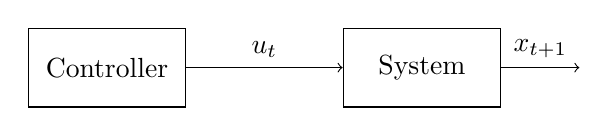
\begin{tikzpicture}[auto, node distance=2cm]
            % Nodes
            \node [draw, rectangle, minimum width=2cm, minimum height=1cm] (control) {Controller};
            \node [draw, rectangle, minimum width=2cm, minimum height=1cm, right of=control, node distance=4cm] (system) {System};
            
            % Arrows
            \draw [->] (control) -- node[above] {$u_t$} (system);
            \draw [->] (system) -- node[above] {$x_{t+1}$} ++(2cm, 0);
    
        \end{tikzpicture}
        \caption{Open Loop Control Strategy}
        \label{fig:block_diagram}
    \end{figure}

    Source: Control bootcamp (Brunton)
    \begin{itemize}
        \item (Dynamical Systems) Systems of ODEs describing state of system has been a successful modeling framework.
        \item Often want to actively make changes to the system. 
        \item In control theory, you have a dynamical system of interest, you write down the system of equations 
        which describes the behavior of the system, and then you create a control theory to create a more ``desireable''
        system behavior.
        \item Passive control (Boyd would call optimal design): design an upfront solution (ex: minimizing drag on a truck)
        \item Active control: pump energy into the system to actively manipulate its behavior.
    \end{itemize}

    \noindent Active Control
    \begin{itemize}
        \item Open Loop
    \end{itemize}

    % \section{Optimal Design}

    % % non stochastic closed loop control
    % \noindent~\cite*{boyd_convex_optimization} \textbf{Exercise 4.17}. \textit{Optimal Activity Levels}.We consider an alternative control application: central planning of some economic activity. It's straightforward to formulate the problem as

    % \[
    % \begin{array}{lll}
    % \text{maximize} \; & \sum_{j=1}^{n}r_j(x_j) & \\
    % \text{subject to} & Ax \preceq c^{\text{max}} &  \\
    % & x \succeq 0. \; & 
    % \end{array}\]
    % However, while the revenue function is a piecewise-linear concave function of the activity
    % level (as stated in the text)

    % \[ r_j(x_j) = \begin{cases}
    %     p_j x_j & 0 \le x_j \le q_j \\
    %     p_j q_j + p_j^{\text{disc}}(x_j - q_j) & x_j \ge q_j,
    % \end{cases}\]
    % this 

    \section{Basic Examples}

    ~\cite{boyd_convex_optimization} \textbf{Exercise 4.16}. \textit{Minimum fuel optimal control}.
    Consider the LTI dynamical system with state $x_t \in \mathbf{R}^n$, $t = 0, \ldots, N$, and actuator
    or input signal $u_t \in \mathbf{R}$, for $t = 0, \ldots, N-1$. The dynamics of the system are governed by the
    linear recurrence
    \[x_{t+1} = Ax_t + bu_t, \quad t=0, \ldots N-1,\]
    where $A \in \mathbf{R}^{m \times n}$ and $b \in \mathbf{R}^n$ are given. Assume the initial state is $x_0 = 0$.
    The \textit{minimum fuel optimal control problem} is to choose the inputs $u_0, \ldots u_{N-1}$ so as to
    minimize the total fuel consumed, which is given by
    \[F = \sum_{t=0}^{N-1}f(u_t),\]
    subject to the constraint that $x_N = x_{\text{des}}$, where $N$ is the (given) time horizon and
    $x_{\text{des}} \in \mathbf{R}^n$ is the (given) desired final or target state. The function $f: \mathbf{R} \to \mathbf{R}$
    is the \textit{fuel use map} for the actuator, and gives the amount of fuel used as a function of the actuator signal amplitude.
    In this problem we use
    \[f(a) = \begin{cases}
        \left| a \right| & \left| a \right| \le 1 \\
        2 \left| a \right| - 1 & \left| a \right| > 1.
        \end{cases}\]
    Formulate the minimum fuel control problem as an LP. 

    \vspace{.1cm}
    \noindent \textbf{Response.}
        Firstly, a few notes about the problem itself:
        \begin{itemize}
            \item ~\cite*{actuator_youtube} What is an actuator (broadly)?
                \begin{itemize}
                    \item A device that makes something move or operate.
                    As a trivial example, an actuator moves the sliding doors at a grocery store.
                    \item Two types: straight line movement (linear) and circular movement (rotary).
                    \item An actuator converts a source of energy into a physical, mechanical motion.
                    A silly example of this: a handwheel can be used to feed energy into a rotary actuator.
                    In industrial applications, there are three typical sources of energy: \textit{Electric} uses electricty (duh),
                    \textit{hydraulic} use a variety of liquids, \textit{pneumatic} are operated by compressed air.
                    \item Common industrial actuators are electric motors, hydraulic motors, and pneumatic control valves.
                    \item Example use of a pneumatic actuator: ``PLC analog output card* produces a 4-20 mA current to move the 
                    valve from fully open to fully closed. The 4-20 mA current will be converted to pneumatic pressure, which
                    becomes the source of energy to operate the actuator.''
                    \item *A Programmable Logic Controller (PLC) analog output card is a component
                    used to convert digital signals from the PLC's processor into analog signals (digital-to-analog conversion, DAC that can
                    be used to control external devices.
                \end{itemize}
            \item Actuator in this problem.
                \begin{itemize}
                    \item $u_t$ is a scalar valued signal that directly affects the state
                    of our system of interest (since it's in the linear recurrence equation).
                    \item Physically, this signal is being used to direct the actuator, which
                    in turn is turning energy into mechanical motion.
                    \item Therefore, the fuel use map for the actuator is a mathematical
                    relation between the amplitude of the signal directing the actuator and
                    the fuel being used. In other words, we can imagine a larger actuator
                    signal corresponds to greater actuator motion, and in this instance,
                    the source of energy needed to produce this motion is ``fuel.''
                \end{itemize}
        \end{itemize}
    % perhaps note that once you establish techniques, you'll stop being explicit with formulations.
     Naive formulation of this problem 
    \[\begin{array}{lll}
    \text{minimize} \; & \sum_{t=0}^{N-1} f(u_t) & \\
    \text{subject to} & x_{t+1} = Ax_t + bu_t \; & t=0, \ldots, N-1 \\
    & x_0 = 0, \quad x_{N} = x_{\text{des}}.
    \end{array}\]
    
    Consider the graph of the fuel use map~\ref{fig:fuel-map}

    % Important/Helpful to map this back to 4.11
    % Actually, how would you map this to ||Ax-b||_1 approximation
    \begin{figure}[h]
        \centering
        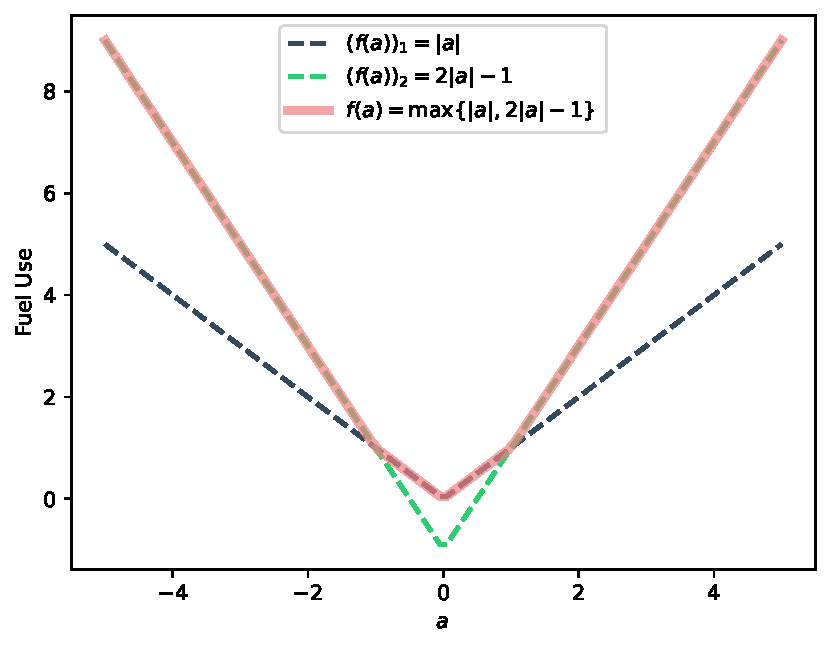
\includegraphics[width=\linewidth]{examples/cvx-ch4/actuator_fuel-use.pdf}
        \caption{Actuator Fuel Use Map.}
        \label{fig:fuel-map}
    \end{figure}

    \[\begin{array}{lll}
        \text{minimize} \; & \sum_{t=0}^{N-1} \max \left\{ \left| u_t \right|, 2 \left| u_t \right| - 1 \right\} & \\
        \text{subject to} & x_{t+1} = Ax_t + bu_t \; & t=0, \ldots, N-1 \\
        & x_0 = 0, \quad x_{N} = x_{\text{des}}.
        \end{array}\]

    \[\begin{array}{lll}
        \text{minimize} \; & \bm{1}^T t & \\
        \text{subject to} & x_{t+1} = Ax_t + bu_t \; & t=0, \ldots, N-1 \\
        & x_0 = 0, \quad x_{N} = x_{\text{des}}, & \\
        & \max \left\{ \left| u_i \right|, 2 \left| u_i \right| - 1 \right\} \le t_i, & i = 0, \ldots, N-1
        \end{array}\]

    \[\begin{array}{lll}
        \text{minimize} \; & \bm{1}^T t & \\
        \text{subject to} & x_{t+1} = Ax_t + bu_t \; & t=0, \ldots, N-1 \\
        & x_0 = 0, \quad x_{N} = x_{\text{des}}, & \\
        & \left| u_i \right| \le t_i, & i = 0, \ldots, N-1 \\
        & 2 \left| u_i \right| - 1 \le t_i & i = 0, \ldots, N-1 \\
        \end{array}\]
    
    \[\begin{array}{lll}
    \text{minimize} \; & \bm{1}^T t & \\
    \text{subject to} & x_{t+1} = Ax_t + bu_t \; & t=0, \ldots, N-1 \\
    & x_0 = 0, \quad x_{N} = x_{\text{des}}, & \\
    & y_i \le t_i, & i = 0, \ldots, N-1 \\
    & 2 y_i - 1 \le t_i & i = 0, \ldots, N-1 \\
    & \left| u_i \right| \le y_i & i = 0, \ldots, N-1 \\
    \end{array}\]
    Important/helpful to remeber the definition of absolute value: $\left| a \right| = \max\{a, -a\}$

    \[\begin{array}{lll}
        \text{minimize} \; & \bm{1}^T t & \\
        \text{subject to} & x_{t+1} = Ax_t + bu_t \; & t=0, \ldots, N-1 \\
        & x_0 = 0, \quad x_{N} = x_{\text{des}}, & \\
        & y_i \le t_i, & i = 0, \ldots, N-1 \\
        & 2 y_i - 1 \le t_i & i = 0, \ldots, N-1 \\
        & -y_i \le u_i \le y_i & i = 0, \ldots, N-1 \\
        \end{array}\]
    Write more compactly as

    \[\begin{array}{lll}
        \text{minimize} \; & \bm{1}^T t & \\
        \text{subject to} & x_{t+1} = Ax_t + bu_t \; & t=0, \ldots, N-1 \\
        & x_0 = 0, \quad x_{N} = x_{\text{des}}, & \\
        & y \preceq t & \\
        & 2y - \bm{1} \preceq t & \\
        & -y \preceq u \preceq y_i & 
        \end{array}\]
    Still not ideal form because of the linear recurrence. Use control theory result.
    
    \begin{figure}[h]
        \centering
        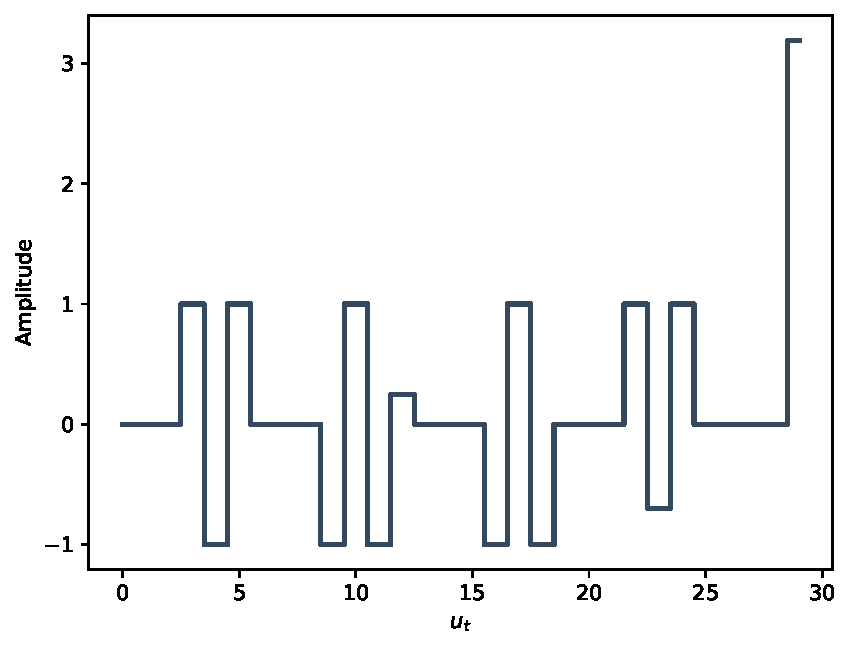
\includegraphics[width=\linewidth]{examples/cvx-ch4/4-16_min-fuel.pdf}
        \caption{Minimum fuel actuator signal.}
        \label{fig:4-16_min-fuel}
    \end{figure}
    
    \vspace*{.5cm}

    \section{Model Predictive Control}

    % Fast MPC: https://web.stanford.edu/~boyd/papers/fast_mpc.html

    \subsection{Overview and Basic Formulations}

    \subsection{Examples}

    % mention that this is a pre real MPC example: no stochasticity
    % list out different variations of MPC

    \subsubsection*{Almost MPC}
    We apply MPC to the following output tracking example. The purpose of this exercise is simply to show
    how sequentially solving receeding horizon problems can converge to the agnostic control problem (where
    the problem is solved with full access to the desired output) as the horizon is increased.
    Note that this example \textbf{does not} demonstrate the power of using MPC in a stochastic setting.

    \noindent~\cite{EE364b} \textbf{HW7 Q1.} \textit{MPC for output tracking}. Consider the linear dynamical system
    \[x_{t+1} = Ax_t + Bu_t, \quad y_t = Cx_t, \quad t = 0, \ldots, T-1,\]
    with state $x_t \in \mathbf{R}^n$, input $u_t \in \mathbf{R}^m$, and output $y_t \in \mathbf{R}^p$.
    The matrices $A$ and $B$ are known, and $x_0=0$. The goal is to choose the input sequence $u_1, \ldots, u_t$
    to minimize the output tracking cost
    \[J_{\text{output}} = \sum_{t=1}^{T}\left\lVert y_t - y_t^{\text{des}} \right\rVert_{2}^2,\]
    subject to $\left\lVert u_t \right\rVert_{\infty} \le U^{\text{max}}, \, t=0, \ldots, T-1$. \\
    For the remainder of this problem we work with the specific problem instance with associated data
    \[A = \begin{bmatrix}
        1 & 1 & 0 \\ 0 & 1 & 1 \\ 0 & 0 & 1
    \end{bmatrix}, \quad
    B = \begin{bmatrix}
        0 \\ 0.5 \\ 1
    \end{bmatrix}, \quad
    C = \begin{bmatrix}
        -1 & 0 & 1
    \end{bmatrix},\]
    $T=100$, and $U^{\text{max}} = 0.1$. The desired output trajectory is given by

    \[y^{\text{des}}_t = \begin{cases}
        0 & t < 30, \\
        10 & 30 \le t < 70 \\
        0 & t \ge 70.
    \end{cases}\]
    (a) Find the optimal input $u^*$ and the associated optimal cost $J^*$.
    
    \vspace{.1cm}
    % is it a linear quadratic tracking problem? What about l_inf constraint?
    \noindent \textbf{Response.} This is simply a \textit{linear} (in the dynamics) \textit{time-invariant quadratic tracking} problem.
    Instead of doing a theoretical analysis of controllability, etc., we can determine the feasibility
    of the control problem by formulating and attempting to solve the following convex optimization problem:
    \[\begin{array}{lll}
    \text{minimize} \; & J_{\text{output}} = \sum_{t=1}^{100}\left\lVert Cx_t - y_t^{\text{des}} \right\rVert_{2}^2 & \\
    \text{subject to} & \left\lVert u_t \right\rVert_{\infty} \le 0.1, \quad x_{t+1} = Ax_t + Bu_t, \; \quad t = 0, \ldots, 99 & \\
    &x_0 = 0,
    \end{array}\]
    (with the provided data for $A$, $B$, $C$, and $y^{\text{des}}$, of course.) Using CVXPY, we obtain the optimal cost 
    $J_{\text{outout}}^{*} = 112.4157$.

    \vspace{.1cm}
    \noindent (b) \textit{Rolling look-ahead}. Now consider the input obtained using an MPC-like method
    where at time $t$, we find the values of $u_t, \ldots, u_{t+N-1}$ that solve the following convex optimization
    problem

    \[\begin{array}{lll}
        \text{minimize} \; & J_{\text{output}} =  \sum_{\tau=t+1}^{t+N}\left\lVert Cx_\tau - y_\tau^{\text{des}} \right\rVert_{2}^2 & \\
        \text{subject to} & \left\lVert u_\tau \right\rVert_{\infty} \le 0.1, \quad x_{\tau+1} = Ax_\tau + Bu_\tau, \; \quad \tau = t, \ldots, t + N - 1 & \\
        &x_0 = 0.
        \end{array}\]
    The value $N$ is the amount of \textit{look-ahead}, since it dictates how much of the future of the desired
    output signal we are allowed to access when we decide on the current input.\\
    Find the input signal for look-ahead values $N=8$, $N=10$, and $N=12$. Compare the cost $J_{\text{output}}$
    obtained in these three instances to the optimal cost $J_{\text{output}}^{*}$ found in part (a).
    
    \vspace{.1cm} 
    \noindent \textbf{Response.} The Python code used to solve this problem can be found in these note's associated examples folder under 364b,
    so it is omitted here. The cost obtained by applying MPC with 
    \begin{itemize}
        \item $N = 8$ is $379.634$,
        \item $N = 10$ is $128.13$,
        \item and $N=12$ is $123.62$.
    \end{itemize}
    Figure~\ref{fig:364-hw7-traj-out} shows the output trajectories for $N=8$, $N=10$, $N=12$,
    the optimal output trajectory, and the desired output trajectory.

    \begin{figure}[h]
        \centering
        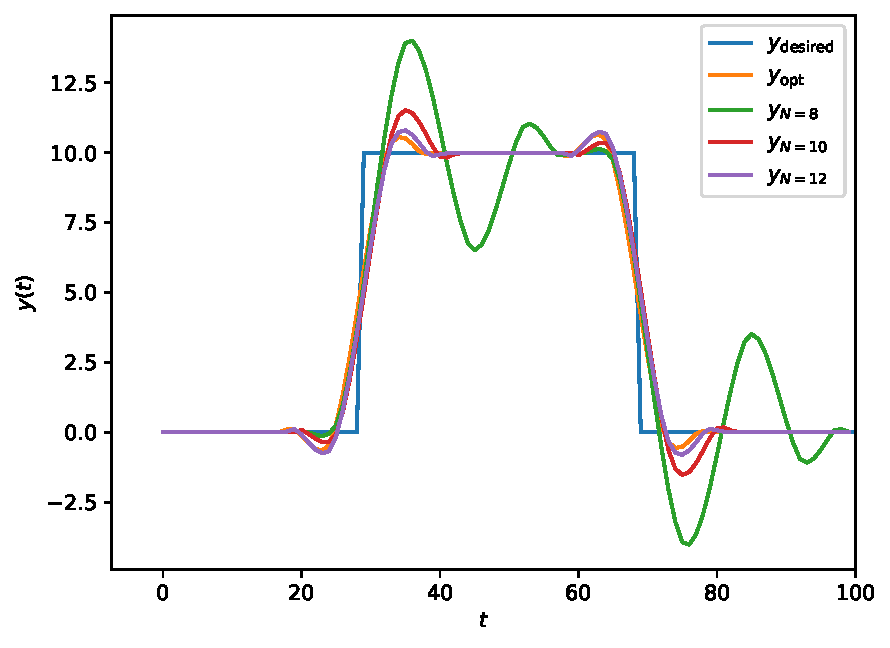
\includegraphics[width=\linewidth]{examples/364b/364b_mpc_output.pdf}
        \caption{Output Trajectories.}
        \label{fig:364-hw7-traj-out}
    \end{figure}
    
\end{chapter}

% Statistical Decision Theory

% Bayesian networks inference (CS221): https://www.youtube.com/watch?v=U23yuPEACG0&t=394s
% sparse Bayes network identification (ex 11.2) https://stanford.edu/class/ee364b/364b_exercises.pdf

% Markov Decision Processes

\part{Algorithms}

\begin{chapter}{Numerical Linear Algebra}

    \section{QR Factorization}
    
    
\end{chapter}

% Sampling and Inference
% Convex Optimization
% Modern (remember that you saw modern Boyd algos in Strang's book)
    % EE364b has GREAT material

% \section*{References}
% \bibliographystyle{apalike}
% \bibliography{refs}
\printbibliography

\appendix

\begin{chapter}{Implementation}

    \begin{itemize}
        \item For now setting is Python.
        \item Will include C++ gradually.
        \item Especially how to generate C optimization solvers from CVXPY.
    \end{itemize}

    \section{CVXPY}
    % my most used library
    % things to keep in mind

    \subsection{Simulating (Linear) Dynamical Systems}

    \section{C++}
    % sliding window: https://www.geeksforgeeks.org/window-sliding-technique/
    % disjoint sets of vertices in a given graph: https://www.geeksforgeeks.org/find-two-disjoint-good-sets-of-vertices-in-a-given-graph/
    % multi threading C++ https://www.geeksforgeeks.org/multithreading-in-cpp/

    % \section{Basic Algebra}

    % \section{Linear Algebra}

    % \begin{itemize}
    %     \item Proof of Cauchy Schwarz
    % \end{itemize}

    % \section{Derivatives}
    % (As a foreward, if it is not said so, assume that a given function is differentiable. When defining new
    % rules and objects I'll attempt to be precise, but elsewhere I may not specify.)

    % \subsection{Matrix Calculus}
    % \subsubsection{Rules}
    % For all the following, assume that $f$ and $g$ are differentiable functions which \textit{make sense} (e.g $f(x)g(x)$
    % where $f$ and $g$ are maps from $\mathbf{R}^n$ to $\mathbf{R}^n$ \textit{would not} make sense
    % as the product of two column vectors is not defined. However, in the same setting $f(x)^T g(x)$ would make sense.)
    % Also, please be careful to remember the notation defined above (In some rules I'll give more context)
    % \begin{enumerate}
    %     \item \textit{Sum Rule}. For $\mathbf{h(x) = f(x) + g(x)}$, $dh = df + dg\; \implies \; Dh(x)dx = Df(x)dx + Dg(x)dx \; \implies \; Dh(x)dx = (Df(x) + Dg(x))dx \; \implies \; \mathbf{Dh(x) = Df(x) + Dg(x)}$
    % \end{enumerate}
    
    % \subsection{Chain rule for second derivative}
    % We'll work on deriving the following case using \textit{matrix calculus} techniques (differentials).
    % \subsubsection*{Composition with scalar function}
    % Suppose $f: \mathbf{R}^n \to \mathbf{R},\; g : \mathbf{R} \to \mathbf{R}$ and $h(x) = g(f(x))$.
    % Finding the first derivative is straightforward: we just utilize the generalized chain rule
    
    % \begin{align*}
    %     Dh(x) = Dg(f(x)) = g'(f(x))Df(x), \label{eq:chain-comp}
    % \end{align*}
    % which implies
    % \begin{align}
    %     \nabla h(x) = g'(f(x))\nabla f(x).
    % \end{align}
    
    % \noindent We now wish to find the \textit{Hessian} of $h$. Recall that for scalar-valued, differentiable functions such as $f$,
    % \[D \nabla f(x) = \nabla^{2}f(x), \]
    % where $\nabla f : \mathbf{R}^n \to \mathbf{R}^n$ is the \textit{gradient mapping} with $\textbf{dom} \, \nabla f = \textbf{dom} \, f$,
    % with value $\nabla f(x)$ at $x$. Furthermore, it's intuitive that the derivative of this gradient mapping is the original function's Hessian.
    % \begin{enumerate}
    %     \item \textit{Intuition Check One} (picture). 
    %     \item \textit{Intuition Check Two} (dimensions). Since the derivative of a function is an (first-order linear approximation)
    %     operator which when given a change in input, outputs the approximate change in the function's input
    % \end{enumerate}

    % We return to \eqref{eq:chain-comp}
    
    % \begin{align*}
    %     d \nabla h = d((g' \circ f) \nabla f )
    % \end{align*}

\end{chapter}
% Remember to add a section with links to things such as "linearizing LPs"

\end{document}